% Name your report <group>-<unique-name>.tex, (e.g., sls-jupiter.tex)
% to avoid name collisions.  For \label{} entries within a file,
% please use \<group>-<unique-name>-<your label} (e.g.,
% \label{sls-jupiter-figure}), again to avoid name collisions.  There
% is no need to use unique names with \cite{} since each report has
% its own citation namespace.

% You can also use \formattitle{Title}{Authors} to gain formatting
% control (e.g., footnotes on author names or controlling line breaks
% with \\) and \formatcontents{Title}{Authors}.  Since we did not need
% such control, we simply used \formattitlecontents{Title}{Authors}
% here.  Please do not put any special formatting in
% \formattitlecontents or \formatcontents as this will disturb the
% table of contents.

\formattitlecontents 
{Linear Analysis and Optimization of Stream Programs}
{Andrew Lamb, William Thies, Saman Amarasinghe}


% Please use the following \formatsection entries unless they are
% inappropriate: Introduction, Approach, Progress, Future, Research
% Support.
%
% Do not put a blank line after a \formatsection, as this affects the
% formatting.
\formatsection{Introduction}
More than fifty percent of the code that runs the Digital Signal Processors
(DSPs) in a modern cell phone is written in assembly language and the 
rest is written in annotated C\cite{gass-talk}. Clearly even the best 
compilers that DSP companies can produce are utterly failing to produce
the necessary level of performance for the programs that run the latest generation
of signal processors.

The sheer volume of analysis required to make optimal use of the special 
purpose architectures available in modern DSPs leaves compilers for existing languages 
floundering. Existing compilers are unable to perform even the simplest 
optimizations taught to undergraduate electrical engineering students. Using 
StreamIt~\cite{streamitcc}, 
a domain-specific stream processing language, we have been exploring
high-level automatic DSP optimizations that are generally impossible
to do in a general-purpose language.

\formatsection{Approach}
Linear analysis and optimization\cite{pldi-03-linear} focuses on
filters which compute {\it linear} functions of their inputs. A filter
computes a linear function if the computation it does can be described
by a vector-matrix multiplication.  Many fundamental DSP operations
such as filtering, the Discrete Fourier Transform (DFT), up sampling
and down sampling, can be described as a vector-matrix
multiplication. The foundation of this project is a simple dataflow
algorithm that can determine which filters in a StreamIt program
perform linear computations and the specific matrices which describe
that computation.

%% \begin{figure}
%%   \begin{minipage}{2.95in}
%%     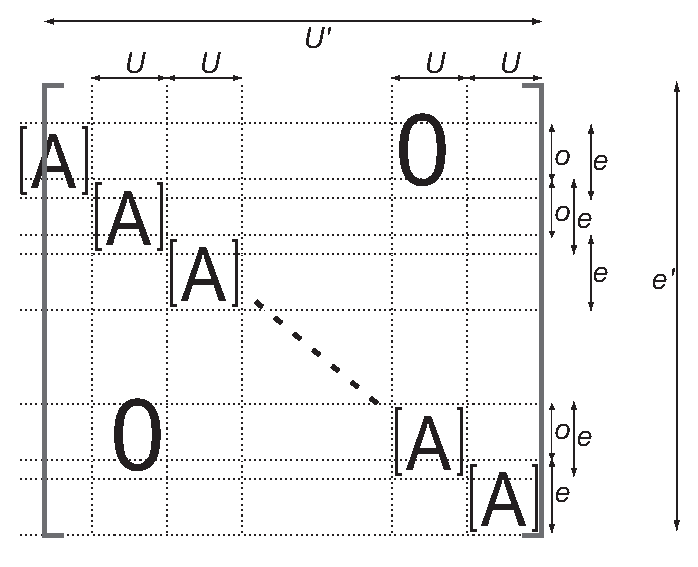
\includegraphics[width=2.8in]{cag-commit-streamit-linear-expand.eps}
    
%% 		    ~~~~~~~{\bf (a) Expanding rates to $(e', o', u')$.}
%%     \end{minipage}
%%     \begin{minipage}{3.3in}
%%       \vspace{0.53in}
%%       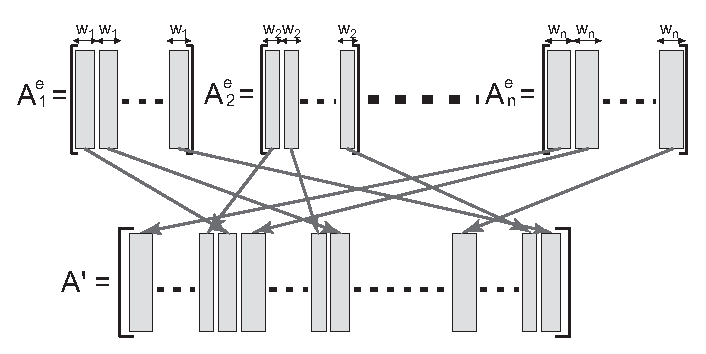
\includegraphics[width=3.25in]{cag-commit-streamit-linear-sjcombo.eps}
%%       \vspace{3pt} \\ 
%%       {\bf (b) Combining a {\tt splitjoin} of linear sub streams.}
%%     \end{minipage}
%%     \caption{Graphical depictions of linear combination algorithms.}
%%     \label{fig:linear-combo}
%%     \vspace{-12pt}
%% \end{figure}

\begin{figure}
\vspace{-12pt}
    \begin{minipage}{2.5in}
      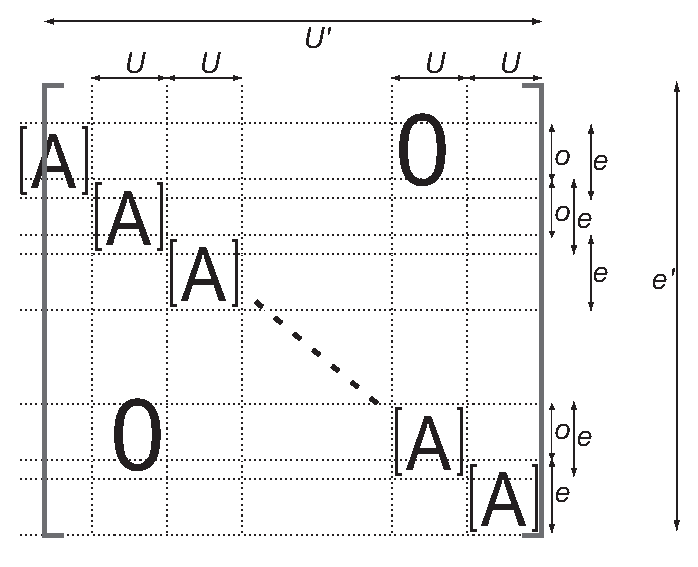
\includegraphics[height=1.6in]{cag-commit-streamit-linear-expand.eps}
      \vspace{-6pt}
      \noindent \caption{Expanding rates to $(e', o', u')$.
        \label{fig:cag-commit-streamit-linear-combo-a}}
    \end{minipage}
    \begin{minipage}{3.5in}
      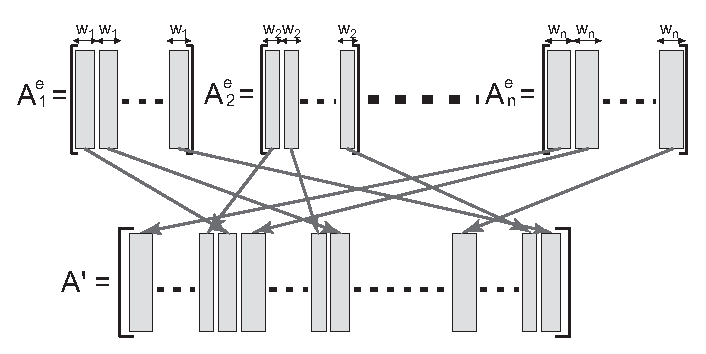
\includegraphics[height=1.6in]{cag-commit-streamit-linear-sjcombo.eps}
      \vspace{-6pt}
      \noindent \protect\hspace{1in}\caption{Combining a {\tt splitjoin} of linear sub streams.
        \label{fig:cag-commit-streamit-linear-combo-b}}
    \end{minipage}
  %%\caption{Graphical depictions of linear combination algorithms.}
  \vspace{-12pt}
\end{figure}

A primary benefit of linear filter analysis is that neighboring
filters can be collapsed into a single matrix representation if both
of the filters are linear. These transformations automatically
eliminate redundant computations in linear sections of the stream
graph. Automating the optimization allows DSP programmers to write
simple, modular filters and leave complex combination and
optimizations to the compiler. Figure~\ref{fig:cag-commit-streamit-linear-combo-a}
illustrates a {\it linear expansion} operation that allows nodes with
mismatching input and output rates to be made compatible before
combining into a single matrix.  Figure~\ref{fig:cag-commit-streamit-linear-combo-b}
depicts the procedure for collapsing $n$ children of a {\tt splitjoin}
construct into a single matrix representation.

To take advantage of the linear analysis framework, our compiler
has two linear analysis optimizations. The first, {\it linear replacement},
replaces the largest possible linear sections of the program with filters
that directly compute the corresponding vector-matrix product. 
The second optimization, {\it frequency replacement}, replaces streams 
which implement digital filtering using a standard conversion to the 
frequency domain.

\formatsection{Progress}
We have developed a fully automatic implementation for linear analysis
and optimization as part of the StreamIt compiler. Our preliminary
results are very promising. For our benchmarks, the optimizations
increased execution speed by an average factor of 5 and a factor of
$6.5$ in the best
case. Figure~\ref{fig:cag-commit-streamit-linear-speedup-a} shows the
speed up for each of the benchmarks.  Both optimizations significantly
reduce the amount of computation required which is reflected by a
reduction in the number of floating point multiplications, shown in
Figure~\ref{fig:cag-commit-streamit-linear-speedup-b}.

\begin{figure}
  \center
  \begin{tabular}{cc}
    \begin{minipage}{3.0in}
      \includegraphics[height=2in]{cag-commit-streamit-linear-speedup.eps}
      \vspace{-12pt}
      \noindent \caption{Execution speedup for each of the benchmarks with both linear 
	replacement and frequency replacement optimizations.
        \protect\label{fig:cag-commit-streamit-linear-speedup-a}}
    \end{minipage} &
    \begin{minipage}{3.0in}
      \includegraphics[height=2in]{cag-commit-streamit-linear-mults.eps}
      \vspace{-6pt}
      \noindent \caption{Percent of multiplication operations remaining after performing 
	linear replacement, frequency replacement, and both.
        \protect\label{fig:cag-commit-streamit-linear-speedup-b}}
    \end{minipage}
  \end{tabular}
  %\caption{Benchmark performance for linear optimizations.}
  %\vspace{-12pt}
\end{figure}

To determine if frequency replacement can fully realize the theoretical maximum 
savings, we measured multiplication reduction as a function
of both filter size and FFT size. It turns out that the theory and the implementation
are very similar. The multiplication reduction predicted by theory are shown in
Figure~\ref{fig:cag-commit-streamit-linear-freq-a} and the reduction that
we measured are shown in Figure~\ref{fig:cag-commit-streamit-linear-freq-b}.

\formatsection{Future}
For future research, we are developing new optimizations which make use
of our linear analysis framework. For instance, we are investigating saving
redundant partial results between filter executions. 
We are also considering expanding our analysis framework to capture
more information about linear computations. Recognizing state variables 
that are linear combinations of the input and previous state would 
allow us to analyze wider range of programs such as adaptive filters 
and control applications.
Another way of extending the framework is to add support for symbolic array entries.
Symbolic entries would allow us to optimize programs which perform
linear operations, but whose coefficient matrices change at runtime.

Finally, we are planning on using the linearity information our
analysis extracts to make more informed decisions in other parts of the compiler.
Furthermore, when the StreamIt compiler targets
a DSP architecture,  we can use the linear information to
take advantage of the specialized instructions offered.

\begin{figure}
  \center
  \begin{tabular}{cc}
    \begin{minipage}{3.0in}
    \begin{center}
      \includegraphics[height=2in]{cag-commit-streamit-linear-freq-theory.eps}
      \vspace{-6pt}
      \noindent \caption{Theoretical multiplication reduction.
        \label{fig:cag-commit-streamit-linear-freq-a}}
      \end{center}
    \end{minipage} &
    \begin{minipage}{3.0in}
    \begin{center}
      \includegraphics[height=2in]{cag-commit-streamit-linear-freq-measure.eps}
      \vspace{-6pt}
      \noindent \caption{Measured multiplication reduction.
        \label{fig:cag-commit-streamit-linear-freq-b}}
	\end{center}
    \end{minipage}
  \end{tabular}
  %%\caption{Theoretical vs. Empirical multiplication reduction.}
  \vspace{-12pt}
\end{figure}

\formatsection{Research Support}
This work is supported by DARPA (PCA F29601-04-2-0166),
the NSF (CISE EIA-0071841), and fellowships from the
Singapore-MIT Alliance and the MIT-Oxygen Project.

% Although the use of BibTeX is highly recommended, you can manually
% format your references as follows:
%
% \begin{thebibliography}{1}
%
% \bibitem{Zue00}
% V.~Zue, S.~Seneff, J.~R. Glass, J.~Polifroni, C.~Pao, T.~J. Hazen, and
% L.~Hetherington, ``\textsc{Jupiter}: A telephone-based conversational
% interface for weather information,'' \textit{IEEE Transactions on
% Speech and Audio Processing}, vol. 8, no.  1, pp. 85--96, Jan. 2000.
% 
% \end{thebibliography}

\bibtex{cag-commit-streamit-linear}
